\documentclass[a4paper]{article}
\usepackage{geometry}
\usepackage{algpseudocode}
\usepackage{algorithm}
\usepackage{algorithmicx}
\usepackage{graphicx}
\usepackage{amsmath}
\usepackage{booktabs}
\usepackage{dsfont}
\usepackage{paralist}
\usepackage{epstopdf}
\usepackage{tabularx}
\usepackage{longtable}
\usepackage{multirow}
\usepackage{multicol}
\usepackage[hidelinks]{hyperref}
\usepackage{fancyvrb}
\usepackage{float}
\usepackage{paralist}
\usepackage[svgname]{xcolor}
\usepackage{enumerate}
\usepackage{array}
\usepackage{times}
\usepackage{url}
\usepackage{fancyhdr}
\usepackage{comment}
\usepackage{environ}
\usepackage{times}
\usepackage{textcomp}
\usepackage{caption}
\usepackage[square,numbers]{natbib}



\urlstyle{rm}



% TO SHOW SOLUTIONS, include following (else comment out):
\newenvironment{soln}{
    \leavevmode\color{blue}\ignorespaces
}{}


\hypersetup{
%    colorlinks,
    linkcolor={red!50!black},
    citecolor={blue!50!black},
    urlcolor={blue!80!black}
}

\geometry{
  top=1in,            % <-- you want to adjust this
  inner=1in,
  outer=1in,
  bottom=1in,
  headheight=3em,       % <-- and this
  headsep=2em,          % <-- and this
  footskip=3em,
}


\title{Gradient Descent for Numerical MAX-CSP} % Title
\author{
Derek Paulsen \\
} 

\date{}

\newcommand{\red}[1]{{\color{red}#1}}
\newcommand{\ind}[1]{\mathds{1}[#1]}
\def \eps{\epsilon}
\begin{document}
\maketitle 


\section{Abstract}
\section{Introduction}

% TODO clean up

Many real world problems can be modeled as constraint 
satisfaction problems. The problems range from logic puzzles 
like sudoku to tuning search engines. Briefly, a constraint satisfaction 
problem is simply the task of finding a valid assignment of variables 
which satisfy as set of constraints. Many classic problems in theoretical computer 
science fit this model, such as the NP-Complete 3-SAT and circuit SAT problems. In this paper 
look variant of CSP, called numerical MAX-CSP. In this variant each variable is a real number
and all of the constraints are linear inequalities, the goal then is to satisfy as 
many linear inequalities as possible. 

The rest of this paper is then structured as follows. First, we give background on the problem 
and the basis for our solution. Next we motivate solving this problem by tying it to 
tuning a keyword search engine with labeled data. We then move on to describe a baseline 
solution by modeling the problem as mixed integer linear program and discuss the issues with 
this solution. Next, we present our algorithm and compare it to the baseline solution. Finally, 
we discuss the experimental results and give directions for future work.

\section{Preliminaries}

In this section we will give an overview of constraint satisfaction problems,
and the specific flavor that we are attempting to tackle in this paper. We then 
give a brief overview gradient descent which is the basis of our proposed solution.

\subsection{Constraint satisfaction problems}

Constraint satisfaction problems (CSPs) encompasses many different problems. Formally a 
constraint satisfaction problem (CSP) is defined as a triple $\langle X, D, C \rangle$ \cite{wiki_CSP}, where 
\begin{align*}
	X &= \{X_1, ..., X_n\} \text{ the set of variables}\\
	D &= \{D_1, ..., D_n\} \text{ the domains of each respective variable}\\
	C &= \{C_1, ..., C_m\} \text{ the set of constraints}\\
\end{align*}
A classic example of a CSP, is the 3-SAT problem. In this case
the boolean variables that appear in at least one clause would be $X$. The domain for 
each variable would be $D_i = \{true, false\}$ and the constraints would all be 
three variable disjunctive clauses. 
In this paper we focus on a subset of CSPs called Numerical MAX-CSP. 
In typical a CSP all constraints must be satisfied, however in MAX-CSP the goal is simply to 
satisfy as may constraints as possible, additionally the domains are the variables 
are numerical (e.g. the real numbers). 

While this problem has certainly been considered before, we were only able to find one previous 
work that directly addresses this issue \cite{num_max_csp_paper}.
In this paper the authors propose a exact solution to numerical MAX-CSP. In particular where 
$D_i = \mathds{R}$ and each constraint $C_j = a_j^Tx \leq b_j, a_j \in \mathds{R}^m, b_j \in \mathds{R}$. 
That is, given a set of linear inequalities, satisfy as many as possible. In the paper the authors 
propose a specific algorithm for this problem based on branch and bound techniques. While the algorithm 
does produce optimal solutions, the algorithm is worst case exponential time.
In fact, this problem is readily to formulated as a mixed integer linear program (MILP),

\begin{align*}
\min_{x,z}\quad &1^Tz\\
s.t. \quad Ax - \epsilon z &\leq b\\
		w &\in \mathds{R}^n\\
		z &\in \{0,1\}^m\\
\end{align*}

Where $\epsilon$ is some large number. The general problem of mixed integer linear programming is 
NP-Hard in general (by reduction to 0-1 integer programming which is NP-Complete \cite{karp_1972}). Hence 
numerical MAX-CSP is likely not to admit an efficient solution. 

\subsection{Gradient Descent}

Gradient descent is an optimization technique which has gained much 
attention in recent years due to the stochastic variant being used in training neural networks for machine learning 
tasks such as computer vision and speech recognition. Despite this focus on machine learning,
gradient descent is a general purpose optimization procedure, capable of optimizing arbitrary 
differentiable functions. Many variations have been proposed in recent years, however
each technique uses the same basic idea. Given a function $f$ and current point $x$, compute $f(x)$. 
Next compute the gradient $\nabla(f(x))$ and update $x$ taking a step in a direction of $-\eta \nabla(f(x))$. Repeat this 
process until the minima of the function is found. 

If $f(x)$ is convex, then gradient descent is guaranteed to find an optimal solution. If $f(x)$ is not convex, 
the gradient descent will converge to a local minimum. Although in the non-convex case, gradient descent 
is not guaranteed, and frequently won't, find the global minimum, it is useful for finding 
minima of functions which are cannot be handled by typical solvers.  This makes it an invaluable tool for 
optimizing functions which don't admit exact optimization techniques such as those used in 
linear programs and quadratic programs.

\section{Motivation}

Numerical MAX-CSPs have a wide variety to applications in such as debugging infeasible 
linear programs, however we are interested in one particular problem, which is that of 
tuning the weights for full search engines. 

Full text search engines are used in a plethora of applications. These search engines (such as Apache Lucene)
are built for efficient retrieval of top-k documents based on a TF/IDF based scoring metric which is dot 
product between two sparse vectors $q^Td = score$\cite{lucene_history} \cite{WAND_paper} \cite{block_max_WAND_paper}.
While this default scoring gives decent results out of the box, 
it is frequently augmented by re-weighting the query $q$, with some weight vector $w$
changing to scoring to be $(q\odot w)^Td = score$. This allows for boosting of certain terms or fields
to improve the quality of search results while not changing the underlying search algorithm. 

The problem we will address in this project is finding a good weight vector $w$. In particular our
problem setting is as follows. We are giving a set of query vectors $Q = \{q_1, ... q_n\}$. For each 
of these query vectors $q_i$ we are given a set of $k$ retrieved document vectors with labels $R_i = \{(d_{i,1}, l_{i,1}), ..., (d_{i, k}, l_{i,k})\}$, 
$l \in \{relevant, irrelevant\}$.
We wish to find a weight vector $w$ that minimizes the number of irrelevant documents that are examined 
before the relevant result is found. This problem can be formulated as a mixed integer linear program (MILP)
as above but with fixed $\gamma < 0$ instead of $b$, in particular,
\begin{align*}
\min_{w,z}\quad &1^Tz\\
s.t. \quad Aw - \epsilon z &\leq \gamma\\
		w &\geq 0\\
		z &\in \{0,1\}\\
\end{align*}

Where each row, $a$, of $A$ comes corresponds to 
$$
a = (d_{i,y} - d_{i,x}) \odot q_i  \quad i \in \{1,...n\} \quad x,y \in \{1,...,k\}, l_{i,x} = relevant, l_{i,y} = irrelevant
$$

That is, the pairwise difference between the components of a matching and non-matching document, multiplied by the 
relevant query. We note that with this setup, 
$$
a^Tw < 0 \implies (q\odot w)^Td_{i,x} > (q\odot w)^Td_{i,y}
$$
That is, the relevant document will be scored higher than the non-relevant document for the query. Solving this 
MILP then corresponds to minimizing the number of irrelevant documents that need to be 
examined in order to find the relevant document for each query. 

\section{Baseline Solution}

As motioned above we can formulate our problem as an  MILP with binary
constraints. This MILP can then be feed into any supported off the shelf solver
to produce an exact optimal answer.  This solution is appealing because,
assuming that the solver is correct, it will give an optimal solution, however
it suffers from a few major drawbacks.  First and foremast, depending on the
input, the solver time could be exponential in the number of constraints.
Moreover we found that even commercial solvers can struggle with large problem
sizes, either taking large amounts of time to produce any feasible solution or
having prohibitive memory requirements.  For our motivating use case, we would
ideally feed in many labeled queries, each producing tens of constraints, hence
exponential runtime in the number of constraints greatly reduces the usefulness
of the solution. 

\section{Our Solution}

To remedy problem of runtime we propose a new solution based on gradient
descent. The high level idea of the solution is simple, begin with a random
weight feasible vector $w$ and then perform gradient descent until the local
minima is found. More specifically we minimize the following function, 

$$
f(w) = \text{HardTanh}(Aw - \gamma)^T\overrightarrow{1}
$$

$$
\text{Where }  \gamma = -1 \text{ and for } x\in R,  \text{HardTanh}(x) = \begin{cases} -1 \text{ if } x \leq -1\\ 1 \text{ if } x \geq 1\\ x \text{ otherwise}\end{cases}
$$

\algrenewcommand\textproc{}
\algrenewcommand{\algorithmiccomment}[1]{\hfill// #1}

\begin{algorithm}[H]
\caption{OptimizeGD($f$, $T$)}
\textbf{Input : } The function $f$ to optimize, a time limit $T$
\textbf{Output : } A local minima $w^*$
\begin{algorithmic}[1]
	\State $w^* \gets \overrightarrow{0}$ 
	\While{current time $ < T$}
		\State $w \gets w \sim \mathds{U}_{[.1,1.1]}^n$ \Comment{Initialize $w$ to a uniform random vector}
		\For{$i =  1,...20$}
			\For{$j =  1,...25$}
				\State $w \gets w - \text{ADAM}(\nabla f(w))$
			\EndFor
			\If{ $f(w) < f(w^*)$}
				\State $w^* \gets w$
			\EndIf
		\EndFor
	\EndWhile
	\\\Return $w^*$
\end{algorithmic}
\end{algorithm}

We use the ADAM optimizer \cite{ADAM_paper} because we emprically found it to perform well,
while giving minimal overhead. 
%TODO add pseduo code?
\section{Experiments}

We ran our experiments on a server with an AMD Ryzen Threadripper 2950X (16c/32t) processor with 
64GB of RAM. Our MAX-CSP instances are generated from real world datasets, with the number of constraints 
ranging from 7.7K to 6.0M. For the baseline solutions we 
leverage Gurobi, a commercial solver with an academic license. We choose gurobi because it is consistently 
one of the top performing available solvers \cite{benchmark}. Both solutions where given a timeout of 2700 seconds 
(corresponding to 24 hours of CPU time).
\begin{table}[ht!]
\caption{Dataset statistics}
\begin{tabular}{|l|r|r|r|}
\toprule
Dataset &  \# of Constraints &  \# of Columns &  \% Non-Zero \\
\midrule
         $D_0$ &                   7.7K &                 14 &         66.24 \\
         $D_1$ &                  19.3K &                 18 &         61.46 \\
         $D_2$ &                 111.9K &                 18 &         72.83 \\
         $D_3$ &                 196.2K &                 30 &         51.62 \\
         $D_4$ &                3.7M    &                124 &         25.09 \\
         $D_5$ &                6.0M    &                 22 &         68.58 \\
\bottomrule
\end{tabular}
\end{table}


\begin{figure}[ht!]
	\caption{Comparison of MILP vs. Gradient Descent (GD)}
	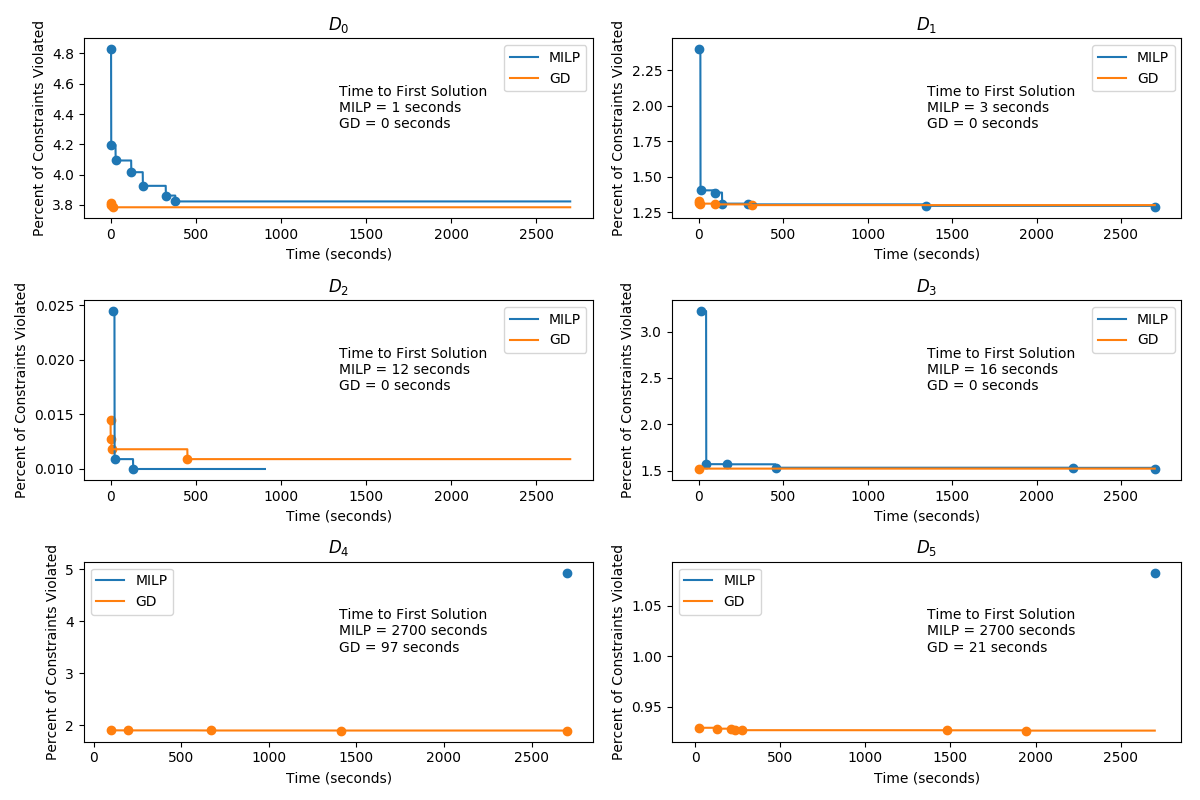
\includegraphics[width=\textwidth]{./time_series.png}
\end{figure}



\section{Discussion}

In this section we will discuss the experimental results. There are
two major points. We first discuss the quality of solutions produced. 
Next, we discuss scalabilty of solutions.

\subsection{Quality of Solutions}

Much to our surprise, the quality of solutions produced by gradient descent
(GD) was very similar if not better than the MILP solution. We attribute this
to the fact that only one dataset was solved to optimality ($D_2$), in fact, we
let $D_0$ run for over 12 hours and MILP still hadn't found an optimal
solution. This was rather suprising because, $D_0$ has less an order of
magnitude fewer constraints than $D_2$. This underlines up a key trade off
between the solutions, namely, quality of solutions vs. runtime predictability.
While the MILP solution will produce optimal solutions given enough time, it is
very hard to predict how long it will take to produce an optimal solution. On
the otherhand, there are no guarantees that can be made about GD in terms of
the quality of solutions but its runtime is very predictable, scaling roughly
linearly with the number of constraints times the number of columns. 

\subsection{Scalability}

This then brings us to our second point which is the scalability of the 
solutions. To begin, from $D_4$ and $D_5$, we can clearly see that 
GD has superior scaling properties when compared to MILP in terms of 
runtime. MILP timed out on both datasets before even begining to refine the 
solutions produced. We attribute this again to the vastly different complexity of the 
two solutions. While GD has linear complexity in the number of constraints, 
MILP has best case polynomial complexity in the number of constraints.  For small 
problems this not an issue, but as the problem size increases MILP quickly becomes
impractical for even approximating the optimal solution. 

\section{Future Work}

We identify multiple directions for future work, which fall into 
two categories, optimization techniques, and problem applications. 

\subsection{Optimization Techniques}

In this paper we have only taken a small look at the possible 
optimization techniques that could be applied. The most obvious 
variation that could tried is to do stochastic gradient descent. This 
variation could have two major potential benefits. First, it can 
decrease both runtime and memory requirements of the solution further by no longer requiring the 
entire dataset be processed on each gradient update. Second, the stochastic 
version may be able to find better solutions as it is much more likely that it 
could escape worse local minima, instead of relying mostly on having a good starting point.


\subsection{Problem Applications}

We restricted our problem setting to numerical MAX-CSPs with linear
constraints, however in principle there is no reason why this technique could
not be applied to arbitrary constraints. In particular, non-convex constraints
would potentially be solved by applying similar techniques, which current
solvers are not able to handle in an capacity. We believe that it is likely
that modifying the optimzation procedure, such as using stochastic gradient
descent, will likely be required to provide good approximations of such
functions.

\section{Conclusion}

In this work we have taken brief look at a particular kind of CSP, namely, 
numerical MAX-CSP's. We motivated this problem with a real world use case for 
tuning full text search engines. We then proposed a solution based on gradient 
descent and gave preliminary evidence to show that it has some key advantages 
over the baseline MILP based solution of the problem, especially for large problem 
sizes where commercial solvers are too slow to practical. We believe that our solution 
shows promise for finding approximate solutions to problems which were not previously tractable
with traditional MILP based solutions. Future work should continue to explore the 
possible variations and possibly apply similar techniques to related problems. 



\bibliographystyle{abbrvnat}
\bibliography{references}
\end{document}
